% =====================================================================
%  Graphical abstract
%  Manifold-Valued Spiking Neurons for Graph Representation Learning
%  (manuscript v38, submitted to Neurocomputing -- Elsevier)
%
%  Elsevier graphical-abstract specification, as applied here
%    * Size: minimum 1328 x 531 px (w x h); the artwork must stay legible
%      when displayed at 13 x 5 cm.  The canvas below is exactly 13 x 5 cm,
%      so the aspect ratio is the required 13:5 and a 300 dpi rasterisation
%      yields 1535 x 591 px -- above the minimum.
%    * File type: PDF / EPS / TIFF preferred.  This source produces a fully
%      vector PDF: no rasterisation, no resolution loss.
%    * Fonts restricted to Times / Arial / Courier / Symbol.  We use newtx,
%      a Times clone, for both text and mathematics.
%    * No heading such as "Graphical Abstract" inside the image, and no
%      separate synopsis file: every label below is baked into the artwork.
%      The title and caption are collected separately by the submission
%      system.
%    * No figure reused from the manuscript: the two data panels are drawn
%      from the same result JSONs but are not copies of any paper figure.
%    * Colour: Okabe-Ito derived (blue / orange / grey).  Blue-orange is
%      distinguishable under red-green colour blindness, and the three fills
%      also differ in value, so the panels survive greyscale printing.
%
%  Layout contract (enforced by check_graphical_abstract.py)
%    * Row 1 (method) occupies y = 3.52 .. 4.74; row 2 (evidence) the rest.
%    * Value labels sit INSIDE the bars.  Placed above the bar tops they
%      collided with the "+10.7" badge; inside there is nothing to hit.
%    * Panel B stacks three bands: heading, bars, takeaway.  The takeaway
%      used to overlap the axis caption, so the caption was folded into the
%      heading and the takeaway moved down.
%
%  Compile:
%      pdflatex graphical_abstract.tex
%
%  Numbers below are read-only reflections of spikergnn_results/:
%      v38_5seeds/{MUTAG,NCI1,PROTEINS,DD}_{OM,MSG}.json
%      v38_euclid/{MUTAG,NCI1,PROTEINS,DD}_EUCLID.json
%  check_graphical_abstract.py re-derives every one of them from the JSONs.
% =====================================================================
\documentclass[tikz,border=0pt]{standalone}

\usepackage[T1]{fontenc}
\usepackage{newtxtext,newtxmath}
\usepackage{xcolor}
\usepackage{tikz}
\usetikzlibrary{arrows.meta,calc,shapes.geometric}

% ---------------------------------------------------------------- colours
\definecolor{com}{HTML}{0F6FA8}    % our model OM          (blue)
\definecolor{cmsg}{HTML}{E08A1E}   % MSG baseline          (orange)
\definecolor{cmech}{HTML}{0F6FA8}  % mechanism effect      (blue)
\definecolor{ccurv}{HTML}{9AA5B1}  % curvature effect      (grey)
\definecolor{ccurvt}{HTML}{5A6675} % curvature text        (dark grey)
\definecolor{cbox}{HTML}{F2F6FA}   % pipeline box fill
\definecolor{cedge}{HTML}{1F5C9C}  % pipeline box edge
\definecolor{ctext}{HTML}{1A2530}
\definecolor{cmuted}{HTML}{6B7A8C}
\definecolor{cgrid}{HTML}{D7DEE6}

% ----------------------------------------------------------------- styles
\tikzset{
  smallf/.style= {font=\fontsize{7}{8.4}\selectfont},
  midf/.style  = {font=\fontsize{7.5}{9}\selectfont},
  pipebox/.style = {draw=cedge, fill=cbox, line width=0.5pt,
                    rounded corners=1.2pt},
  pipearr/.style = {-{Stealth[length=1.5mm, width=0.9mm]},
                    line width=0.7pt, draw=cedge},
}

\begin{document}
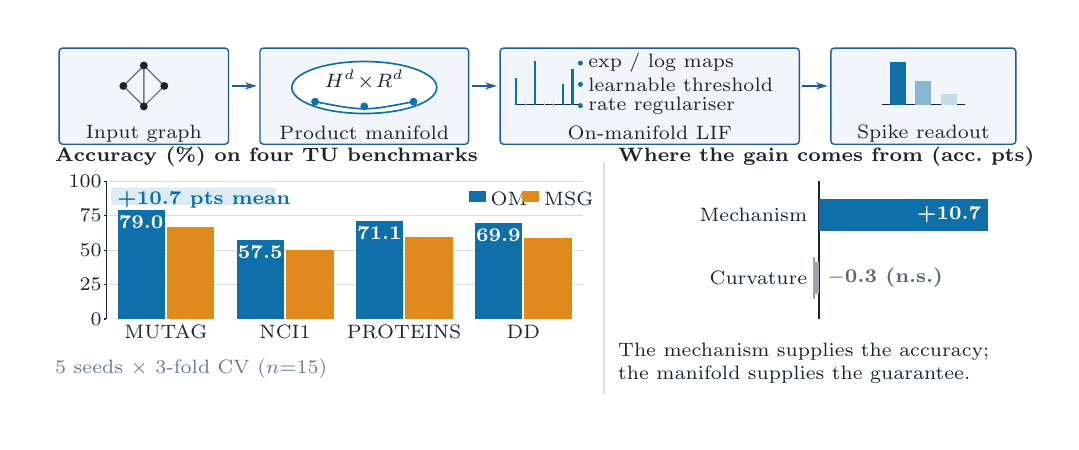
\begin{tikzpicture}[x=1cm, y=1cm, inner sep=0pt, outer sep=0pt]

% =====================================================================
%  Canvas -- pins the standalone crop box to exactly 13 cm x 5 cm.
% =====================================================================
\fill[white] (0,0) rectangle (13,5);

% =====================================================================
%  ROW 1 -- the method, read left to right   (band y = 3.52 .. 4.74)
% =====================================================================

\draw[pipebox] (0.40, 3.52) rectangle (2.55, 4.74);   % input graph
\draw[pipebox] (2.95, 3.52) rectangle (5.60, 4.74);   % product manifold
\draw[pipebox] (6.00, 3.52) rectangle (9.80, 4.74);   % on-manifold LIF
\draw[pipebox] (10.20,3.52) rectangle (12.55,4.74);   % spike readout

\draw[pipearr] (2.59,4.26) -- (2.91,4.26);
\draw[pipearr] (5.64,4.26) -- (5.96,4.26);
\draw[pipearr] (9.84,4.26) -- (10.16,4.26);

% ---- box 1: input graph ----------------------------------------------
\draw[cmuted, line width=0.5pt]
      (1.475,4.52) -- (1.215,4.26) -- (1.475,4.00) -- (1.735,4.26) -- cycle
      (1.475,4.52) -- (1.475,4.00);
\foreach \p in {(1.475,4.52),(1.215,4.26),(1.475,4.00),(1.735,4.26)}
  \fill[ctext] \p circle (0.05);
\node[smallf, ctext] at (1.475,3.66) {Input graph};

% ---- box 2: product manifold -----------------------------------------
%  A disk carrying a geodesic arc: the state lives ON the manifold.
\fill[white] (4.275,4.24) ellipse [x radius=0.92, y radius=0.33];
\draw[com, line width=0.6pt]
      (4.275,4.24) ellipse [x radius=0.92, y radius=0.33];
\draw[com, line width=0.6pt]
      (3.65,4.06) .. controls (4.275,3.94) .. (4.90,4.06);
\fill[com] (3.65,4.06)  circle (0.05);
\fill[com] (4.275,4.00) circle (0.05);
\fill[com] (4.90,4.06)  circle (0.05);
\node[midf, ctext] at (4.275,4.34) {$\mathbb{H}^{d}\!\times\!\mathbb{R}^{d}$};
\node[smallf, ctext] at (4.275,3.66) {Product manifold};

% ---- box 3: on-manifold LIF, plus the three mechanisms ---------------
\draw[ctext, line width=0.4pt] (6.20,4.02) -- (7.00,4.02);
\foreach \x in {6.20, 6.32, 6.44, 6.56, 6.68, 6.80, 6.92}
  \draw[cgrid, line width=0.5pt] (\x,4.02) -- (\x,4.08);
\foreach \x/\h in {6.20/0.34, 6.44/0.56, 6.80/0.26, 6.92/0.46}
  \draw[com, line width=0.9pt] (\x,4.02) -- (\x,4.02+\h);

\foreach \y in {4.55, 4.28, 4.01}
  \fill[com] (7.02,\y) circle (0.032);
\node[smallf, ctext, anchor=west] at (7.12,4.55) {exp / log maps};
\node[smallf, ctext, anchor=west] at (7.12,4.28) {learnable threshold};
\node[smallf, ctext, anchor=west] at (7.12,4.01) {rate regulariser};
\node[smallf, ctext] at (7.90,3.66) {On-manifold LIF};

% ---- box 4: spike-gated readout --------------------------------------
\draw[ctext, line width=0.4pt] (10.85,4.02) -- (11.90,4.02);
\fill[com]    (10.95,4.02) rectangle (11.15,4.57);
\fill[com!50] (11.275,4.02) rectangle (11.475,4.32);
\fill[com!25] (11.60,4.02) rectangle (11.80,4.16);
\node[smallf, ctext] at (11.375,3.66) {Spike readout};

% =====================================================================
%  ROW 2 -- the evidence
% =====================================================================
\draw[cgrid, line width=0.5pt] (7.32,0.35) -- (7.32,3.30);

\node[smallf, ctext, anchor=south west] at (0.35,3.24)
      {\bfseries Accuracy (\%) on four TU benchmarks};
\node[smallf, ctext, anchor=south west] at (7.50,3.24)
      {\bfseries Where the gain comes from (acc.\ pts)};

% ---------------------------------------------------------------- PANEL A
%  Grouped bars: OM against the tangent-space MSG baseline.
%  Axis is 0-100 % (not truncated): plot band y = 1.30 .. 3.05,
%  i.e. 0.0175 cm per accuracy point.  The band stops at 3.05 so that the
%  "100" tick clears the panel heading above it.
\foreach \v/\y in {0/1.30, 25/1.7375, 50/2.175, 75/2.6125, 100/3.05} {
  \node[smallf, ctext, anchor=east] at (0.94,\y) {\v};
  \draw[ctext, line width=0.4pt] (0.97,\y) -- (1.00,\y);
}
\foreach \y in {1.7375, 2.175, 2.6125, 3.05}
  \draw[cgrid, line width=0.3pt] (1.00,\y) -- (7.05,\y);
%  The unit lives in the panel heading rather than in a rotated axis label:
%  a rotated label at x=0.50 collided with the "100" tick, and the heading
%  already sits directly above the axis.
\draw[ctext, line width=0.5pt] (1.00,1.30) -- (1.00,3.05);

\fill[com]  (1.141,1.30) rectangle (1.741,2.6825);   % MUTAG    OM  79.0
\fill[cmsg] (1.771,1.30) rectangle (2.371,2.4638);   % MUTAG    MSG 66.5
\fill[com]  (2.654,1.30) rectangle (3.254,2.3063);   % NCI1     OM  57.5
\fill[cmsg] (3.284,1.30) rectangle (3.884,2.1750);   % NCI1     MSG 50.0
\fill[com]  (4.166,1.30) rectangle (4.766,2.5443);   % PROTEINS OM  71.1
\fill[cmsg] (4.796,1.30) rectangle (5.396,2.3430);   % PROTEINS MSG 59.6
\fill[com]  (5.679,1.30) rectangle (6.279,2.5233);   % DD       OM  69.9
\fill[cmsg] (6.309,1.30) rectangle (6.909,2.3273);   % DD       MSG 58.7

%  Values sit inside the bars -- see the layout contract in the header.
\node[smallf, white] at (1.441,2.5225) {\bfseries 79.0};
\node[smallf, white] at (2.954,2.1463) {\bfseries 57.5};
\node[smallf, white] at (4.466,2.3843) {\bfseries 71.1};
\node[smallf, white] at (5.979,2.3633) {\bfseries 69.9};

\node[midf, ctext, anchor=north] at (1.756,1.22) {MUTAG};
\node[midf, ctext, anchor=north] at (3.269,1.22) {NCI1};
\node[midf, ctext, anchor=north] at (4.781,1.22) {PROTEINS};
\node[midf, ctext, anchor=north] at (6.294,1.22) {DD};

%  legend
\fill[com]  (5.60,2.79) rectangle (5.82,2.93);
\node[smallf, ctext, anchor=west] at (5.88,2.83) {OM};
\fill[cmsg] (6.28,2.79) rectangle (6.50,2.93);
\node[smallf, ctext, anchor=west] at (6.56,2.83) {MSG};

%  headline gain
\fill[com!14, rounded corners=1pt] (1.06,2.75) rectangle (3.16,2.97);
\node[midf, com, anchor=west] at (1.14,2.81) {\bfseries +10.7 pts mean};

\node[smallf, cmuted, anchor=south west] at (0.35,0.55)
      {5 seeds $\times$ 3-fold CV ($n{=}15$)};

% ---------------------------------------------------------------- PANEL B
%  Diverging bars: how much of the gain the mechanism and the curvature
%  each account for.  Both rows share one scale, 0.20 cm per point.
\draw[ctext, line width=0.7pt] (10.05,1.30) -- (10.05,3.05);

\fill[cmech] (10.05,2.42) rectangle (12.19,2.82);
\node[midf, white, anchor=east] at (12.11,2.62) {\bfseries +10.7};
\node[midf, ctext, anchor=east] at (9.90,2.62) {Mechanism};

%  The curvature bar is deliberately almost invisible: at 0.20 cm per point
%  the -0.3 point effect is 0.6 mm wide.  The tick marks it so the reader
%  can see there IS a bar, and the number carries the magnitude.
\fill[ccurv] (9.99,1.62) rectangle (10.05,2.02);
\draw[ccurv, line width=0.8pt] (9.99,1.55) -- (9.99,2.09);
\node[midf, ccurvt, anchor=west] at (10.16,1.82) {\bfseries $-$0.3 (n.s.)};
\node[midf, ctext, anchor=east] at (9.90,1.82) {Curvature};

\node[smallf, ctext, anchor=north west] at (7.50,1.00)
      {The mechanism supplies the accuracy;};
\node[smallf, ctext, anchor=north west] at (7.50,0.70)
      {the manifold supplies the guarantee.};

\end{tikzpicture}
\end{document}
